\section{Software Performance} \label{chapter3:software-performance}

% The previous section showed that modular programming limits performance scalability of execution.




\subsection{Concurrency}





The criteria to analyze the solutions presented in this section are :
\begin{itemize}
\item fine level sequentiality
\item coarse level message passing
\end{itemize}

The sequentiality of execution at a fine level assures the invariance on the shared state.
The message passing used assures the independence, and immutability at a coarser level of execution, hence the parallelism.
Both these organizations are needed to 


\begin{figure}[h!]
\begin{center}
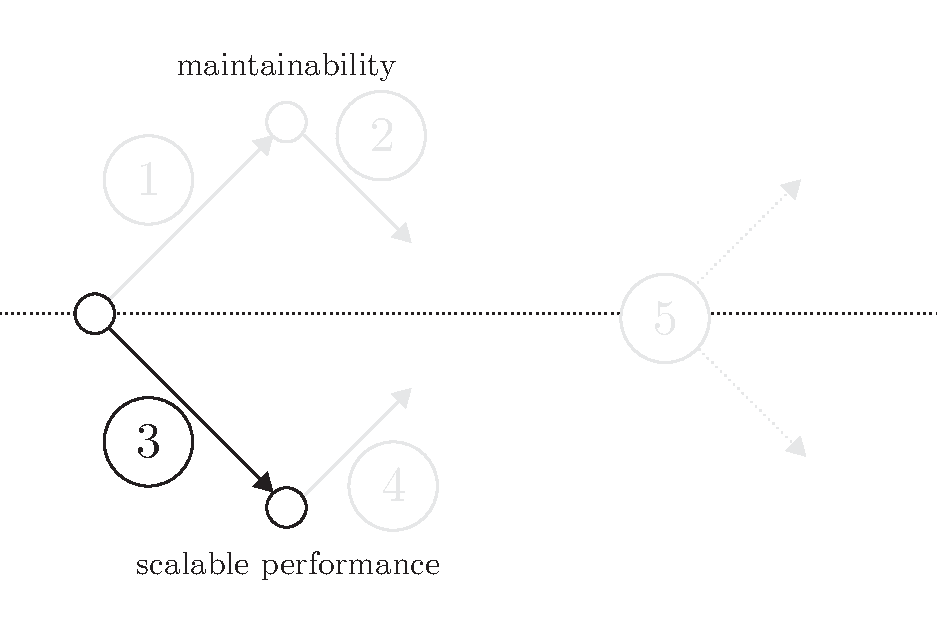
\includegraphics[width=0.6\textwidth]{../ressources/state-of-the-art-3.pdf}
\end{center}
\end{figure}



\subsubsection{Concurrent Programming} \label{chapter3:software-maintainability:concurrency:concurrent-programming}

% \cit{Building concurrent programming is like building a steam engine through a keyhole}{TODO}

IMPORTANT -> Synchronization at a coarse grain is bad for performance.

Concurrent programming provides to the developer the mechanisms for concurrent execution, while conserving a global memory model.

\illustration{feu rouge et rond point}

There are two scheduling strategies to execute tasks sequentially on a single processing unit, cooperative scheduling and preemptive scheduling.
Cooperative scheduling allows a concurrent execution to run until it yields back to the scheduler.
Each concurrent execution has an atomic, exclusive access on the memory.
On the other hand, preemptive scheduling allows a limited time of execution for each concurrent execution, before preempting it.
It assures fairness between the tasks, such as in a multi-tasking operating system, but as the preemption happens unexpectedly it breaks atomicity, the developer needs to lock the shared state to assure atomicity and exclusivity.
The next paragraphs presents the event-driven programing model, based on cooperative scheduling, and the multi-threading programming model, based on preemptive scheduling.

\nt{and then lock-free data-structures}

\paragraph{Event-Driven Programming}

Event-driven programming explicitly queues the concurrent executions needing access to shared resources.
The concurrent executions are schedule sequentially to assure exclusivity, and cooperatively to assure atomicity.

\comment{As presented in the previous chapter, }web servers needs to be highly concurrent, and efficient.
The event-driven model is very efficient to serve websites, as it avoids contention due to waiting for shared resources like disks, or network.
Web servers like Flash \cite{Pai1999}, Ninja \cite{Gribble2001} thttpd\ftnt{http://acme.com/software/thttpd/} and Nginx\ftnt{https://www.nginx.com/} were designed following this model.
However, a drawback of this model was that the execution context is lost at each event.
The developer needs to explicitly transfer the relevant state to continue the execution from one event execution to another.

Cooperative threads, or fibers, addressed this drawback \cite{Adya2002,Behren2003a}.
The execution is not ripped into several events.
It yields and resume exactly at the same point after the completion of an asynchronous operation, conserving its context.
However, the developer needs to be well aware of the asynchronous calls to assure the atomicity\ftnt{https://glyph.twistedmatrix.com/2014/02/unyielding.html}.\nt{more about that, it is important, and transition with the next}
% + Fibers \cite{Adya2002}
% + Capricio \cite{Behren2003a} - User cooperative threads (also known as fibers / green threads)

The problem of losing the execution context disappears with closures in higher-order programming.
\nt{link with the previous paragraph}
Moreover, the continuation passing style used in higher-order programming requires the developer to be aware of the asynchronous rupture in the execution, so as to assure atomicity \cite{Sussman1998}.
And because an asynchronous call doesn't wait for the completion of the operation, the asynchronous control flow is not limited to be linear like in threads. \nt{more about that}
Multiple asynchronous calls are made in parallel.
Several execution model proposed this event-based programming model, like TAME \cite{Krohn2007}, Node.js\ftnt{https://nodejs.org/en/} and Vert.X\ftnt{http://vertx.io/}.
% + TAME \cite{Krohn2007} - event-based solution without stack ripping in C (it is like closure, but for C)
% + Node.js - \ftnt{https://nodejs.org/en/}
% + Vert.X - \ftnt{http://vertx.io/} node like + thread / worker capabilities

However, as the shared memory is global and all the execution portions needs atomic access, they are not parallel, but sequentially concurrent.
The next paragraph present the multi-threading and associated synchronization mechanisms to try improve the parallelism of execution using finer granularity of atomic execution and exclusivity.

\paragraph{Multi-Threading Programming}

Threads are light processes sharing the same memory execution context within an isolated process \cite{Dijkstra1968}.
They wait for completion of each operation, and are preemptively scheduled to avoid blocking the global progression.
This preemption breaks the atomicity of the execution, and the parallel execution breaks the exclusivity.
To restore atomicity and exclusivity, hence assure the invariance, multi-threading programming model provide synchronization mechanisms, such as semaphores \cite{Dijkstra}, guarded commands \cite{Dijkstra1975}, guarded region \cite{Hansen1978a} or monitors \cite{Hoare1974}.
They assure an execution region to have exclusive access over a cell of the global state.

\cit{The purpose of explicit synchronization is to manage the timing of side-effects in the presence of parallelism.}{Chris Quenelle\ftnt{http://pchiusano.blogspot.com/2010/01/actors-are-not-good-concurrency-model.html?showComment=1267337235223\#c3014836700278061280}}

Developers tend to use the global memory extensively, and threads require to protect each and every shared memory cell.
This heavy need for synchronization leads to bad performances, and is difficult to develop with \cite{Adya2002}.
The next paragraph present work intending to improve performance by reducing the lock granularity to a minimum.

\nt{Add Fork-join parallelism : Cilk \cite{Randall1998,Frigo1998,Leiserson2010}}

\paragraph{Lock-Free Data-Structures}

The wait-free and lock-free data-structures reduce the exclusive execution to a few atomic operations \cite{Lamport1977,Herlihy1988,Herlihy1990,Herlihy1991,Anderson1990}.
They are based on transactional memories \cite{Harris2010}, which provide atomic read and write operations on a shared memory.
Lock-free data-structures arrange these atomic operations so as to keep invariance without the need to lock.
They provide concurrent implementation of basic data-structures such as linked list \cite{Valois1995,Timnat2012}, queue \cite{Sundell2003,Wimmer2015}, tree \cite{Ramachandran2015} or stack \cite{Hendler2004}.

However, even if they are theoretically infinitely scalable, they are hard to come with, and are not fit for every problem.

\nt{Fork-join parallelism : Cilk \cite{Randall1998,Frigo1998,Leiserson2010}}

% Reference papers :
% Concurrent reading and writing \cite{Lamport1977}
% Impossibility and universality results for wait-free synchronization \cite{Herlihy1988}
% A methodology for implementing highly concurrent data structures \cite{Herlihy1990}
% Wait-free synchronization \cite{Herlihy1991}

% Book :
% The virtue of Patience: Concurrent Programming With And Without Waiting \cite{Anderson1990}



\begin{table}[h!]
\label{maintainability-scalability}
\small
\begin{tabu} to \linewidth {@{} l X[l] c c c c @{}}
%
% \multicolumn{3}{c}{}  & \rot{Concurrency} & \multicolumn{2}{|c}{Parallelism} \\
Model & Implementations    & \rot{Fine level sequentiality} & \rot{Coarse level message passing} & $\to$ & \rot{Scalability} \\
\tabucline[.5pt]{-}
%                                                                               SEQ  MSG   SCL
Event-driven programming       & Node.js, Vert.X                               & \V & \X && \X \\ \tabucline[on .5pt]{-}
Multi-threading programming    & Lock, Mutex, Semaphores, Guarded regions      & \V & \X && \X \\ \tabucline[on .5pt]{-}
Lock-free Data Structures      &                                               & \V & \X && \X \\
\tabucline[.5pt]{-}
\end{tabu}
\caption{Analysis of the state of the art regarding concurrent programming}
\end{table}


\paragraph{}



Moore's law \cite{Moore1965} which forecasts the density of transistors per processing unit, was wrongly interpreted to promise the exponential evolution in the sequential performance of the processing unit, and the assurance for the software industry of always faster hardware.
But as transistors attained a critical size, the reduction in power required by transistor predicted by the Dennard's MOSFET scaling \cite{Dennard2007} stopped\ftnt{https://cartesianproduct.wordpress.com/2013/04/15/the-end-of-dennard-scaling/}.
The ever growing number of transistor predicted by Moore's law are arranged in parallel architecture to continue increasing the performance of processing units.
Parallel programming became the only solution for scalable performance, at the expense of development effort.

This section presents the parallel programming solutions and their limitations in accessibility, and then the improvements to overcome these limitations.




Concurrent programming is a compromise to keep shared states, while introducing different forms of synchronization to keep the execution sequential.
But because of the lack of clear isolation, the execution is not parallel, hence the performance is limited.


\nt{The shared-nothing architecture \cite{Stonebraker1986}}


\subsubsection{Parallel Programming} \label{chapter3:software-performance:parallel-programming}


Concurrent programming is based on the causal ordering of execution.
The ordering of operations is local within a synchronous execution, while the concurrent executions are causally ordered.
It leads to parallel execution with some coordinations such as synchronization, immutability or isolation.
As Lamport showed \cite{Lamport1978}, and Reed related later \cite{Reed2012}, This causal order is sufficient to execute correctly a system in parallel, such as in distributed system.

This section presents first hand the theoretical and programming model based on asynchronous communication and isolated execution for parallel programming, as illustrated on the schema above.
It then continues with stream processing programming model. 
And finally,it concludes on the limitations of parallel programming regarding accessibility. 


\nt{read and include The Landscape of Parallel Computing Research: a view from berkeley, by Asonovic, Bodik, Catanzaro, Gebis, Husbands, Keutzer ...}


\paragraph{Asynchronous and Isolated Process Parallelism}

The Flynn's taxonomy \cite{Flynn1972} is the most commonly used to categorize parallel execution.
It separates the flow of instructions, and the flow of data ; each being unique, or multiple.
All the current parallel programming model currently belong to the category Multiple Instruction Multiple Data (MIMD), which is further divided into Single Program Multiple Data (SPMD) \cite{Auguin1983,Darema1988,Darema2001} and Multiple Program Multiple Data (MPMD) \cite{Chang1997,Chan2004}.
MIMD implies several threads of execution processing several stream of data.
% The difference between SPMD and MPMD holds on the distinction of instruction pool between the threads of execution.
% SPMD implies to replicate the same program on all the processing units, while MPMD implies to define different programs for every processing units.

% \begin{figure}
% \begin{center}
% 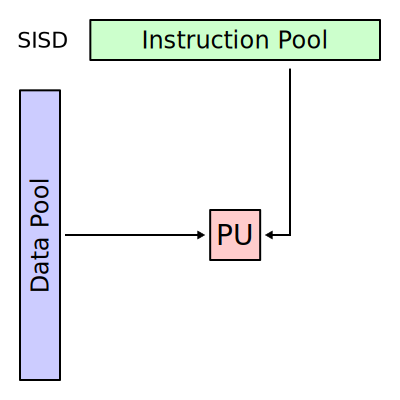
\includegraphics[width=0.2\textwidth]{../ressources/SISD.svg}
% 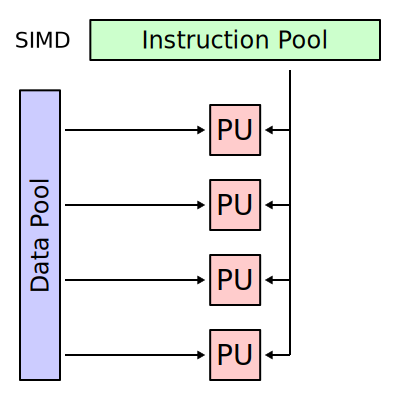
\includegraphics[width=0.2\textwidth]{../ressources/SIMD.svg}
% 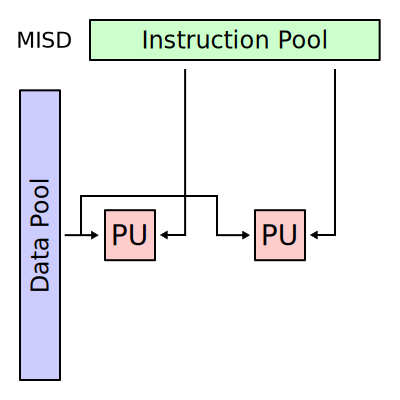
\includegraphics[width=0.2\textwidth]{../ressources/MISD.svg}
% 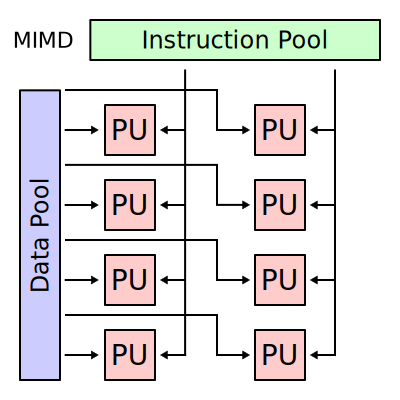
\includegraphics[width=0.2\textwidth]{../ressources/MIMD.svg}\\
% by I, Cburnett. Licensed under CC BY-SA 3.0 via Commons
% \url{https://commons.wikimedia.org/wiki/File:SISD.svg#/media/File:SISD.svg}
% \url{https://commons.wikimedia.org/wiki/File:SIMD.svg#/media/File:SIMD.svg}
% \url{https://commons.wikimedia.org/wiki/File:MISD.svg#/media/File:MISD.svg}
% \url{https://commons.wikimedia.org/wiki/File:MIMD.svg#/media/File:MIMD.svg}
% \end{center}
% \nt{TODO convert these svg to pdf}
% \caption{Flynn's taxonomy of parallelism}
% \end{figure}

\nt{schemas SPMD / MPMD}

SPMD -> concurrent programming, multi-threading and so on ...
MPMD -> Actor model based programming

The difference between SPMD and MPMD is in the representation of the execution in implementation.
SPMD organizes the implementation as a single execution replicated on many processing units.
While MPMD organizes explicitly the different threads of execution in the implementation.
Examples of SPMD programming languages are
Split-C \cite{Culler},
CRL \cite{Johnson1995} and
Composite C++ \cite{K.ManiChandy2005}.
%
Examples of MPMD programming languages are
Mentat \cite{Grimshaw1991},
Fortran M \cite{Foster1995b} and
Nexus \cite{Foster1996}.
SPMD is close to the model presenting parallel improvements over modular programming presented in section \ref{chapter3:software-maintainability:programming-models}.
While MPMD is closer to the programming models based on isolated process presented in the remaining of this section.
The coordinations between these threads of execution were done by message passing, using PVM \cite{Sunderam1994}, MPI \cite{Snir1996,Walker1996}, SOAP, or the more recent REST protocols.

\subparagraph{Theoretical Models}

The communication in reality are subject to various faults and attacks \cite{Lamport1982} and too slow compared to execution to be synchronous.
The Actor model is one of the first programming model to be explicitly designed to take these physical limitations in account \cite{Hewitt1977a}.
It allows to express the computation as a set of communicating actors \cite{Hewitt1973a, Hewitt1977, Clinger1981}.
In reaction to a received message, an actor can create other actors, send messages, and choose how to respond to the next message.
All actors are executed concurrently, and communicate asynchronously.
An asynchronous communication implies that the sender continues its execution immediately after sending the message, before receiving the result of the initiated communication.

In the Actor Model, everything is an actor, even the simplest types like numbers.
This level of granularity is unachievable in practice due to overhead from the asynchronous communications.
Most implementations adopt a granularity on the process or function level.

Coroutines are autonomous programs which communicate with adjacent modules as if they were input and output subroutines \cite{Conway1963}.
It is the first definition of a pipeline to implement multi-pass algorithms.
Similar works include the Communicating Sequential Processes (CSP) \cite{Hoare1978, Brookes1984}, and the Kahn Networks \cite{Kahn1974, Kahn1976}.

\begin{table}[h!]
\label{maintainability-scalability}
\small
\begin{tabu} to \linewidth {@{} l X[l] c c c c @{}}
%
% \multicolumn{3}{c}{}  & \rot{Concurrency} & \multicolumn{2}{|c}{Parallelism} \\
Model & Implementations    & \rot{Fine level sequentiality} & \rot{Coarse level message passing} & $\to$ & \rot{Scalability} \\
\tabucline[.5pt]{-}
%                                                                               SEQ  MSG   SCL
Event-driven programming       & Node.js, Vert.X                               & \V & \X && \X \\ \tabucline[on .5pt]{-}
Multi-threading programming    & Lock, Mutex, Semaphores, Guarded regions      & \V & \X && \X \\ \tabucline[on .5pt]{-}
Lock-free Data Structures      &                                               & \V & \X && \X \\
\tabucline[.5pt]{-}
Actor Model                    & Scala, Akka, Play, Erlang                     & \V & \V && \V \\
\tabucline[.5pt]{-}
\end{tabu}
\caption{Analysis of the state of the art regarding scalability}
\end{table}

\subsection{Organic Growth}


A system is maintainable only if there is competences available to maintain it.

The criteria to analyze the solutions presented in this section regarding the organic growth are : 
\begin{itemize}
\item adoption by the community
\item adoption by the industry
\item supporting web technologies
\end{itemize}
The first two criteria make sure that the technology is growing organically with a passionate community, and backed by industrial needs.
The last criteria assures the fitting of the technologies with our economical context of a web application. 

\begin{figure}[h!]
\begin{center}
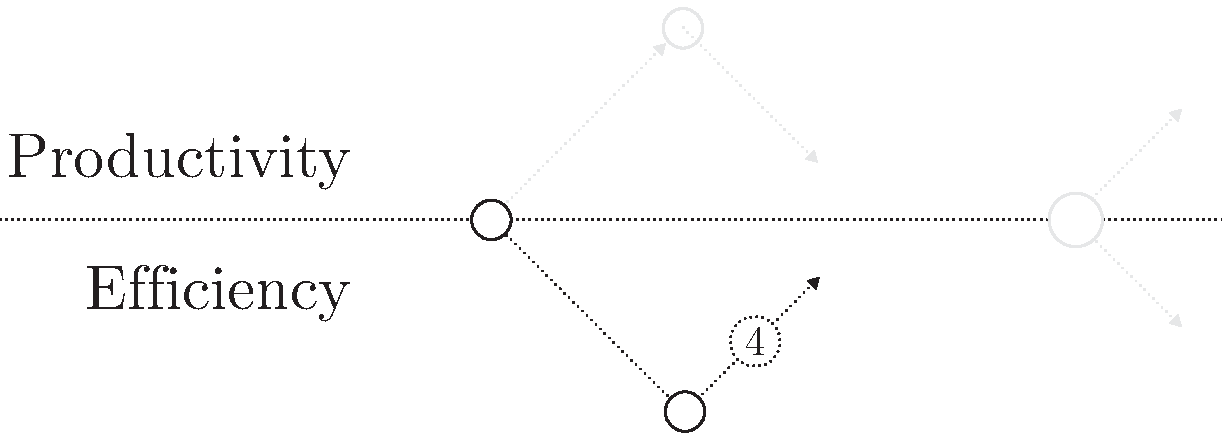
\includegraphics[width=0.6\textwidth]{../ressources/state-of-the-art-4.pdf}
\end{center}
\end{figure}


\subsubsection{Programming Languages}

The theoretical models presented above are implemented in industrial languages such as Akka Scala and Erlang \cite{JoeArmstrong} .

Scala is an attempt at unifying the object model, and functional programming \cite{Odersky2004}.
% It proposes an actor approach in its design.
Akka\ftnt{http://akka.io/} is a framework based on Scala, following the Actor model to build higly scalable and resilient applications.
Play\ftnt{https://www.playframework.com/} is a web framework based on top of Akka.

Erlang borrow the Actor model as well.
It is a functional concurrent language designed by Ericsson to operate telecommunication devices \cite{JoeArmstrong,Nelson2004} % Nelson2004 is not very good, find another better citation.

\nt{review this paragraph and the transition to the next section}
The field of concurrent programming is so vast it is impossible to relate here every programming languages.
The previous examples are only the best known.
The next focus focuses on streaming real-time applications.

% \comment{transition on lazy evaluation equivalence to stream. lazy evaluation + side effects + concurrency = streams}


+ all the solutions that have a great industrial impact (storm, millwheel and co)

Eventually, the research merges with the academy at some level, because the need for performance is higher than the need for maintainability.
Industries have the money to pay researchers, great engineers and so on ...



\subsubsection{Execution Organization}


\paragraph{Stream Processing Systems}

All the solutions previously presented are designed to build general distributed systems.
In the context of the web, a real-time application must process high volumes streams of requests within a certain time.
Because these systems are key to business, their reliability and latency are of critical importance.
Otherwise, input data may be lost or output data may lose their value.
These requirements are challenging to meet in the design of such system.

\subparagraph{Data-stream Management Systems}

Database Management Systems (DBMS) historically processed large volume of data, and they naturally evolved into Data-stream Management System (DSMS) to processed data streams as well.
Because of this evolution, they are in rupture with imperative languages presented until now, and borrow the syntax from SQL.

DSMS concurrently run SQL-like requests on continuous data streams.
The computation of these requests spread over a distributed architecture.
Among the early works, we can cite
NiagaraCQ \cite{Chen2000,Naughton2001},
Aurora \cite{Abadi2003,Abadi2003a,Balakrishnan2004} which evolved into
Borealis \cite{Abadi2005},
AQuery \cite{Lerner2003},
STREAM \cite{Arasu2003,Arasu2005} and
TelegraphCQ \cite{Krishnamurthy2003,Chandrasekaran2003}.
More recently, we can cite
DryadLINQ \cite{Isard2007,Yu2009},
Apache Hive \cite{Thusoo2009}\ftnt{https://hive.apache.org/},
Timestream \cite{Qian2013} and
Shark \cite{Xin2013}.


\subparagraph{Pipeline Architecture}

As presented in the previous section, streaming and lazy-evaluation composition both allow a loosely coupled yet efficient composition.
The pipeline architecture takes advantage of this, and composes the parallel execution in a stream, the output of one feeding the input of the next.

SEDA is a precursor in the design of pipeline-based architecture for real-time web applications \cite{Welsh2001}.
It organizes an application as a network of event-driven stages connected by explicit queues.
The event-driven paradigm is similar to previous web servers implementations like Ninja and Flash \cite{Gribble2001,Pai1999}.
SEDA improves with the pipeline organization in stages.

Several projects followed and adapted the principles in this work.
StreaMIT is a language to help the programming of large streaming application \cite{Thies2002}.
Storm \cite{Toshniwal2014} is designed by and used at Twitter to process the heavy streams of tweets.
% It is only one example of industrial practical application, among many others.
Among other works, in the industry, there are
CBP \cite{Logothetis2010} and
S4 \cite{Neumeyer2010}, that were designed at Yahoo,
Millwheel \cite{Akidau2013} designed at Google and
Naiad \cite{Murray2013} designed at Microsoft.

In the litterature, there are
Spidle \cite{Consel2003},
Pig Latin \cite{Olston2008},
Piccolo \cite{Power2010},
Comet \cite{He2010},
Nectar \cite{Gunda2010},
SEEP \cite{Migliavacca2010},
Legion \cite{Bauer2012},
Halide \cite{Ragan-Kelley2013},
SDG \cite{Fernandez2014a} and
Regent \cite{Slaughter2015}




All of the parallel programming models presented above decompose the execution into isolated parallel executions, like actors.
This decomposition is difficult as it implies to manage both the parallel decomposition of execution and the modular decomposition of implementation.
Most developers are unable to manage efficiently the two decompositions.
The next paragraphs presents some solutions to mitigate this duality.
\nt{TODO weak argumentation}

\paragraph{Design Patterns}

To reduce the difficulties of the decomposition of the execution into actors, algorithmic skeletons propose predefined patterns that fit certain type of problems \cite{Cole1988, Dean2008, McCool2010, Gonzalez-Velez2010}.
A developer implements the problem as a specific case of a skeleton.
It simplifies the communications, so that the developer can focus on its problem independently of message passing required by the distribution of execution.

% \nt{Link with DSMS}
% As there is similtudes between SQL-like languages, functional structures, and algorithmic skeletons, the latter can be seen as a tentative to merge the more descriptional features of the former into imperative programming.
% Indeed, among the Algorithmic skeletons, we can cite Map / reduce, which are functional structures, but are somehow equivalent to the select and aggregate functions of SQL.
% The pipeline architecture for data stream processing presented in section \ref{chapter3:software-efficiency:dataflow-pipeline} can be considered as algorithmic skeletons.

% However, they introduce limitations and difficulties, as the developer must fit its problem into the skeletons.
% One of this difficulties, it that a common memory is impossible to use.
% Developers needs to think in terms of message passing instead of a global memory, which, as we saw in previous section, is incompatible with best practices.

% Introducing 'Bones': a parallelizing source-to-source compiler based on algorithmic skeletons \cite{Nugteren2012}

\paragraph{Granularity}

The Service Oriented Architectures (SOA), and more recently Microservice\cite{Namiot2014,Fernandez-Villamor2010,Fowler2014,Namiot2014} allow developers to express an application as an assembly of services connected to each others.
Some examples of frameworks are OSGi\ftnt{https://www.osgi.org/developer/specifications/}, EJB\ftnt{http://www.oracle.com/technetwork/java/javaee/ejb/index.html}, Spring\ftnt{http://projects.spring.io/spring-framework/}, and Seneca\ftnt{http://senecajs.org/}
It intends to adjust the granularity of execution decomposition to help developers to fit the two organizations, the modular organization and the parallel execution organization \cite{Adam2008}.

% In modular programming a module protects the rest of the implementation from the consequences of the design choice its encapsulate, while a service encapsulate a specific task, with possible consequences on the adjacent services.

% In a fine enough granularity of service, each service becomes so simple, it can limits the consequences of its modification.







\subsubsection{Usage}


TODO


\begin{table}[h!]
\label{maintainability-scalability}
\small
\begin{tabu} to \linewidth {@{} l X[l] c c c c c @{}}
%
% \multicolumn{3}{c}{}  & \rot{Concurrency} & \multicolumn{2}{|c}{Parallelism} \\
Model & Implementations    & \rot{Community adoption} & \rot{Industrial adoption} & \rot{Web compliant} & $\to$ & \rot{Growth} \\
\tabucline[.5pt]{-}
% %                                                                               COM  IND  WEB   GRO
Event-driven programming       & Node.js, Vert.X                               & \V & \V & \V && \V \\ \tabucline[on .5pt]{-}
Multi-threading programming    & Lock, Mutex, Semaphores, Guarded regions      & \X & \V & \V && \V \\ \tabucline[on .5pt]{-}
Lock-free Data Structures      &                                               & \X & \V & \V && \V \\
\tabucline[.5pt]{-}
Actor Model                    & Scala, Akka, Play, Erlang                     & \X & \V & \X && \X \\ \tabucline[on .5pt]{-}
Data Stream System Management  & DryadLINQ \cite{Isard2007,Yu2009},%
                                 Apache Hive \cite{Thusoo2009}\ftnt{https://hive.apache.org/},%
                                 Timestream \cite{Qian2013},%
                                 Shark \cite{Xin2013}.                         & \X & \V & \X && \X \\ \tabucline[on .5pt]{-}
Pipeline Stream Processing     & SEDA, Storm, Spark Streaming,%
                                 Spidle \cite{Consel2003},%
                                 Pig Latin \cite{Olston2008},%
                                 Piccolo \cite{Power2010},%
                                 Comet \cite{He2010},%
                                 Nectar \cite{Gunda2010},%
                                 SEEP \cite{Migliavacca2010},%
                                 Legion \cite{Bauer2012},%
                                 Halide \cite{Ragan-Kelley2013},%
                                 SDG \cite{Fernandez2014a},%
                                 Regent \cite{Slaughter2015}.                  & \X & \V & \V && \X \\
\tabucline[.5pt]{-}
\end{tabu}
\caption{Analysis of the state of the art regarding organic growth}
\end{table}

\subsection{Maintainability Limitations}


\nt{to integrate
In these parallel programming models describing a network of isolated execution, the topology of the network is statically defined. 
The dynamical modification of the topology is impossible.
It is not possible to dynamically manipulate execution containers, like it is possible to manipulate functions.
Therefore, higher-level programming is impossible, so modular programming is limited.
%
Moreover, the decomposition of the execution and memory required is difficult for most developers to manage correctly.
TODO make sure this idea is correctly developed throughout this chapter : parallel programming implies to keep a double mental representation.
It implies to keep two mental representation of the implementation.
One for the modularity, and one for the decomposition of execution.
Parallel programming remains hard, and is accessible only to an elite of developers.
%
% \subsubsection{Lack of Higher-Order Programming}
The programming models of this section lack higher order programming.
% Moreover, in these solutions, higher-order programming is impossible.
As showed earlier in section \ref{chapter3:software-design:programming-models:functional-programming}, higher-order programming is important for modular design and maintainability of the implementation.
In this regards, parallel programming seems currently incompatible with modular programming.
The next section presents the proposition of this thesis to bring parallel programming to a higher-order programming language.
% By keeping the modular programming model, the compilation approach allows higher-level programming.
% \paragraph{Transistion : these methods doesn't allow higher-order programming, which is required for good modularity. WHY ?}
% \nt{TODO link with 3.1}
}


Because of the hybridization of state access, a granularity of sharing appears.
At a fine level, the state is shared, while at a coarser level, it is isolated.
Because of this difference, programming languages abandoned shared state, and higher-order programming between execution containers.
These two features are responsible for the modularity of Functional Programming and Object Oriented Programming models.

To allow a continuous development of a web service, a language must present these three features :

\begin{itemize}
\item scalability
\item maintainability
\item abstract the decomposition
\end{itemize}

The first allows the evolution of the performance.
The second assure the evolution of the implementation.
The third is required to allow these two first features to coexist.



\begin{table}[h!]
\label{maintainability-scalability}
\small
\begin{tabu} to \linewidth {@{} l X[l] c c c @{}}
%
% \multicolumn{3}{c}{}  & \rot{Concurrency} & \multicolumn{2}{|c}{Parallelism} \\
Model & Implementations    & \rot{Memory decomposition abstraction} & $\to$ & \rot{Maintainability} \\
\tabucline[.5pt]{-}
%                                                                               ABS   MAI
Event-driven programming       & Node.js, Vert.X                               & \V && \V \\ \tabucline[on .5pt]{-}
Multi-threading programming    & Lock, Mutex, Semaphores, Guarded regions      & \X && \X \\ \tabucline[on .5pt]{-}
Lock-free Data Structures      &                                               & \X && \X \\
\tabucline[.5pt]{-}
Actor Model                    & Scala, Akka, Play, Erlang                     & \X && \X \\ \tabucline[on .5pt]{-}
Data Stream System Management  & DryadLINQ \cite{Isard2007,Yu2009},%
                                 Apache Hive \cite{Thusoo2009}\ftnt{https://hive.apache.org/},%
                                 Timestream \cite{Qian2013},%
                                 Shark \cite{Xin2013}.                         & \X && \X \\ \tabucline[on .5pt]{-}
Pipeline Stream Processing     & SEDA, Storm, Spark Streaming,%
                                 Spidle \cite{Consel2003},%
                                 Pig Latin \cite{Olston2008},%
                                 Piccolo \cite{Power2010},%
                                 Comet \cite{He2010},%
                                 Nectar \cite{Gunda2010},%
                                 SEEP \cite{Migliavacca2010},%
                                 Legion \cite{Bauer2012},%
                                 Halide \cite{Ragan-Kelley2013},%
                                 SDG \cite{Fernandez2014a},%
                                 Regent \cite{Slaughter2015}.                  & \X && \X \\
\tabucline[.5pt]{-}
\end{tabu}
\caption{Analysis of the state of the art regarding maintainability}
\end{table}


\subsection{Summary}

\begin{table}[h!]
\label{maintainability-scalability}
\small
\begin{tabu} to \linewidth {@{} l X[l] c c c @{}}
%
% \multicolumn{3}{c}{}  & \rot{Concurrency} & \multicolumn{2}{|c}{Parallelism} \\
Model & Implementations    & \rot{Modularity} & \rot{Organic Growth} & \rot{Scalability} \\
\tabucline[.5pt]{-}
%                                                                               MOD  GRO  SCA
Event-driven programming       & Node.js, Vert.X                               & \V & \V & \X \\ \tabucline[on .5pt]{-}
Multi-threading programming    & Lock, Mutex, Semaphores, Guarded regions      & \X & \V & \V \\ \tabucline[on .5pt]{-}
Lock-free Data Structures      &                                               & \X & \V & \V \\
\tabucline[.5pt]{-}
Actor Model                    & Scala, Akka, Play, Erlang                     & \X & \X & \V \\ \tabucline[on .5pt]{-}
Data Stream System Management  & DryadLINQ \cite{Isard2007,Yu2009},%
                                 Apache Hive \cite{Thusoo2009}\ftnt{https://hive.apache.org/},%
                                 Timestream \cite{Qian2013},%
                                 Shark \cite{Xin2013}.                         & \X & \X & \V \\ \tabucline[on .5pt]{-}
Pipeline Stream Processing     & SEDA, Storm, Spark Streaming,%
                                 Spidle \cite{Consel2003},%
                                 Pig Latin \cite{Olston2008},%
                                 Piccolo \cite{Power2010},%
                                 Comet \cite{He2010},%
                                 Nectar \cite{Gunda2010},%
                                 SEEP \cite{Migliavacca2010},%
                                 Legion \cite{Bauer2012},%
                                 Halide \cite{Ragan-Kelley2013},%
                                 SDG \cite{Fernandez2014a},%
                                 Regent \cite{Slaughter2015}.                  & \X & \X & \V \\
\tabucline[.5pt]{-}
\end{tabu}
\caption{Summary of the analysis of the state of the art}
\end{table}

\endinput







TO READ :

Streaming
\cite{Madsen2015}
\cite{Sun2015}

Map Reduce
\cite{Yao2015}


Web assembly
https://medium.com/javascript-scene/what-is-webassembly-the-dawn-of-a-new-era-61256ec5a8f6












\endinput

\subsection{Concurrency Theory} \label{chapter3:parallel-execution:concurrency-theory}

The mathematical models are a ground for all following work on concurrent programming, we briefly explain them in the next paragraphs.
There are two main formal models for concurrent computations.
The Actor Model of C. Hewitt and the Pi-calculus of R. Milner.
Based on these definitions, we explain the importance of determinism for correctness, and the reasons that made asynchronous message-passing prevail.

% TODO illustration of cells, and draw an analogy between cells and actor model.
% Or something the actor models is based upon.

\subsubsection{Models}

\paragraph{Actor Model}

The Actor model allows to express the computation as a set of communicating actors \cite{Hewitt1973a, Hewitt1977, Clinger1981}.
In reaction to a received message, an actor can create other actors, send messages, and choose how to respond to the next message.
All actors are executed concurrently, and communicate asynchronously.
% The Actor model uses an asynchronous message-passing communication paradigm.
% The communication between two actors, the sender and the receiver, is a stream of discrete messages.
% The sender names the receiver actor when sending messages to be the recipient of these messages.
An asynchronous communication implies that the sender continues its execution immediately after sending the message, before receiving the result of the initiated communication.

The Actor model was presented as a highly parallel programming model, but intended for Artificial Intelligence purposes.
Its success spread way out of this scope, and it became a general reference and influence.
% For example, the Scala programming language features an actor approach to concurrency.

% More recent work of C. Hewitt on Actors is about ... \nt{TODO} \cite{Hewitt2007,Hewitt2007a}.

\paragraph{$\pi$-calculus}

R. Milner presented a process calculus to describe concurrent computation : the Calculus of Communicating Systems (CCS) \cite{Milner1975, Milner1980}.
It is an algebraic notation to express identified processes communicating through synchronous labeled channels.
% In CCS, process compose concurrently, communications are synchronous, and the topology is static.
The $\pi$-calculus improved upon this earlier work to allow processes to be communicated as values, hence to become mobile \cite{Engberg1986,Milner1992a,Milner1992}.
Therefore, similarly to Actors, in Pi-calculus processes can dynamically modify the topology.
However, contrary to the Actor model, communications in Pi-calculus are based on simultaneous execution of complementary actions, they are synchronous.


% Actors can create actors, pi-caclulys processes can replicate, and send processes through channel.
% Processes create a new processes on each instruction to continue the execution.!g systolic arrays

% Pi-calculus resembles to the actor model, but its algebraic nature led to a critical difference with the latter.
% Indeed, processes in the Pi-calculus communicate indirectly, through labeled ports, whereas actors communicate directly by naming the recipient actors.
% This difference allows multiple processes to listen in turns to the same channel, whereas the recipient of a message cannot change.

% I think this difference lead the Pi-calculus to be composable, whereas message-passing is not.
% Message-passing is not composable, whereas invocation is.
% The Actor model is not an ideal programming model, as non-composability makes difficult to reuse or extends existing components.
% A way to compose actors, is to send to an actor the name of the actor to respond to.
% It is similar in essence to the continuation concept.








\section{Reconciliations} \label{chapter3:reconciliations}
\nt{TODO title not clear enough}

\subsection{Contradiction}

The decomposition of an application into a pipeline, as shown in the two previous sections, is incompatible with the modular design advocated by the separation of concerns.
The problem of incompatibility between the modular design and the parallel execution of a pipeline architecture is the following.
There need to be a common understanding on the structure of the communication from one stage to the next.
The modular design defines that this common ground, the interface, be the most resilient possible to focus the evolution within a module.
While the pipeline architecture (and more generally the concurrent programming models) defines these interfaces as the communications between the stages of the execution.
With the evolution of the problem specification, when a stage needs to be modified, it is most likely that these changes will affect the previous or next stages.
% which will eventually change with the evolution of the problem specification.

Most project use languages supporting the modular design at the beginning, when they need to evolve the most.
They then switch to the pipeline architecture only when the requirement of performance overcomes the requirement of evolution.
Moreover, as the team knows that they will eventually throw away their code to upgrade it to a different paradigm, there is little effort to follow the best practice to make maintainable code.
It results in a large effort of development to compensate this rupture.
% This rupture between the two organization is not novel, and is at the center of a large body of work.
In this section, we present the state of the art to reconciliate the two organizations, and avoid this rupture.
First we see the design patterns to fit both organization onto a same source code.
Then we see the compilation tentatives to switch from one to the other.